% Standalone: "Standard Attention" panel — QK and OV side by side, each with its
% per-channel quantity written underneath (QK: attention score; OV: per-token transfer).
% Convention: query on the LEFT, key on the RIGHT (matches x_q W_QK x_k^T read left-to-right).
% Compile: pdflatex fig_attn_standard.tex
\documentclass[tikz,border=3pt]{standalone}
\usepackage[T1]{fontenc}
\usepackage{newtxtext,newtxmath}
\usepackage{microtype}
\usepackage{tikz}
\usetikzlibrary{arrows.meta,positioning,calc}

\definecolor{ink}       {HTML}{172033}
\definecolor{greyLine}  {HTML}{9CA3AF}
\definecolor{greyFill}  {HTML}{F3F4F6}
\definecolor{qkC}       {HTML}{B91C1C}
\definecolor{ovC}       {HTML}{0B7285}

\tikzset{
  >={Latex[length=2.5mm,width=1.8mm]},
  panel/.style={draw=greyLine,line width=0.7pt,rounded corners=4pt,
    fill=white,inner sep=3mm},
  title/.style={font=\large\bfseries,text=ink,align=center},
  smalltitle/.style={font=\normalsize\bfseries,text=ink,align=center},
  poslabel/.style={font=\normalsize\bfseries,text=ink,align=center},
  greySubBox/.style={draw=greyLine,line width=0.75pt,rounded corners=3pt,
    fill=white,inner sep=3mm},
  greyFeat/.style={draw=greyLine,line width=0.7pt,rounded corners=1.5pt,
    fill=greyFill,minimum width=10mm,minimum height=8mm,inner sep=1pt,
    font=\normalsize\bfseries,text=ink},
  greyUnknown/.style={draw=greyLine,line width=0.7pt,rounded corners=1.5pt,
    fill=greyFill,minimum width=10mm,minimum height=16mm,inner sep=1pt,
    font=\normalsize\bfseries,text=ink},
  eq/.style={font=\Large,text=ink,align=center},
}

\begin{document}
\begin{tikzpicture}[x=1mm,y=1mm]
\node[panel,fill=greyFill,minimum width=130mm,minimum height=86mm,anchor=north west] (pa) at (0,80) {};
\node[title] at (pa.north) [yshift=-4.5mm] {Standard Attention};

% --- QK sub-box (left): query -> key, right-facing ---
\node[greySubBox,minimum width=58mm,minimum height=42mm,anchor=north west] (stdQK) at ([xshift=1.5mm,yshift=-8.5mm]pa.north west) {};
\node[smalltitle,text=qkC] at ([yshift=-4mm]stdQK.north) {QK: where to attend};
\node[greyUnknown] (stdQ1) at ([xshift=-17mm,yshift=-24mm]stdQK.north) {?};
\node[greyUnknown] (stdK1) at ([xshift=17mm,yshift=-24mm]stdQK.north) {?};
\draw[->,line width=1.2pt,greyLine] (stdQ1.east) -- (stdK1.west);
\node[poslabel] at ([yshift=-2.5mm]stdQ1.south) {query};
\node[poslabel] at ([yshift=-2.5mm]stdK1.south) {key};

% --- OV sub-box (right) ---
\node[greySubBox,minimum width=58mm,minimum height=42mm,anchor=north east] (stdOV) at ([xshift=-1.5mm,yshift=-8.5mm]pa.north east) {};
\node[smalltitle,text=ovC] at ([yshift=-4mm]stdOV.north) {OV: what to move};
\node[greyUnknown] (stdV) at ([xshift=-17mm,yshift=-24mm]stdOV.north) {?};
\node[greyFeat,minimum width=13mm] (stdOut) at ([xshift=17mm,yshift=-24mm]stdOV.north) {out};
\draw[->,line width=1.2pt,greyLine] (stdV.east) -- (stdOut.west);
\node[poslabel] at ([yshift=-2.5mm]stdV.south) {value};

% --- per-channel math, centered between sub-box bottom and panel bottom ---
\node[eq,anchor=center] at ($(stdQK.south)!0.5!(stdQK.south |- pa.south)$)
  {$\displaystyle A^{h}_{qk}=\tfrac{1}{\sqrt{d_h}}\; x_{q} W^{h}_{QK}\, x_{k}^{\top}$};
\node[eq,anchor=center] at ($(stdOV.south)!0.5!(stdOV.south |- pa.south)$)
  {$\displaystyle \mathrm{OV}^{h}_{k}=W^{h}_{OV}\, x_{k}$};
\end{tikzpicture}
\end{document}
